
\documentclass{jtetiproposalskripsi}

%-----------------------------------------------------------------
%Disini awal masukan untuk data proposal tugas akhir
%-----------------------------------------------------------------
\titleind{PERANCANGAN SISTEM APLIKASI MANAJEMEN SURAT MENGGUNAKAN PHP FRAMEWORK CODEIGNITER 
 DAN CSS TWITTER BOOTSTRAP DI KANTOR PGRI KABUPATEN JEMBER}
\fullname{IIS DAHLIA}

\idnum{1200631047}

\approvaldate{14 Januari 2015}

\degree{Diploma Manajemen Informatika}

\yearsubmit{2015}

\program{Manajemen Informatika}

\headprogram {Sarjiya, S.T., M.T., Ph.D.}

\dept{}

\firstsupervisor{Triawan Adi Cahyanto,M.Kom}
\firstnip{12 03 719}

\secondsupervisor{Bagus Setya Rintyarna,S.T,M.Kom}
\secondnip{09 03 521}


%-----------------------------------------------------------------
%Disini akhir masukan untuk data proposal skripsi
%-----------------------------------------------------------------

\begin{document}

\cover
 
\approvalpage

%-----------------------------------------------------------------
%Disini akhir masukan untuk muka skripsi
%-----------------------------------------------------------------

%-----------------------------------------------------------------
%Disini awal masukan Intisari
%-----------------------------------------------------------------
\begin{abstractind}
Seiring dengan pesatnya perkembangan teknologi informasi saat ini menuntut suatu organisasi atau instansi dalam membutuhkan teknologi Informasi. Banyak kegiatan yang hanya dapat dilakukan pada lingkup terbatas menjadi cakupan yang sangat luas sampai mendunia. Dengan keberadaan pengolahan data menjadi sistem informasi secara terkomputerisasi. Hal ini dikarenakan pengolahan data secara terkomputerisasi dapat memberikan kontribusi yang besar untuk kinerja suatu organisasi utamanya dibidang pengarsipan surat keluar masuk.
Dengan menggunakan fitur yang dimiliki sistem informasi berbasis web, yang dapat dimanfaatkan sebagai sistem keamanan pengarsipan surat keluar masuk pada instansi. Banyak fitur-fitur unggulan yang dimiliki web untuk merancang suatu sistem dimana salah satunya dapat menggunakan PHP Framework Codeigniter dan CSS Twitter Bootstrap yang dikonfigurasikan menjadi elemen-elemen sistem informasi aplikasi surat berbasis web dengan desain yang lebih dinamis dan kelebihan dari Framework Codeigniter dengan kecepatan yang diintegrasikan menjadi sistem yang lebih baik.

\begin{flushleft}

\textbf{Kata Kunci} : \textit{Aplikasi Manajemen Surat Masuk dan Keluar, PHP Framework Codeigniter dan CSS Twitter Bootstrap}
\end{flushleft}

\bigskip

\end{abstractind}
%-----------------------------------------------------------------
%Disini akhir masukan Intisari
%-----------------------------------------------------------------

\tableofcontents
\addcontentsline{toc}{chapter}{DAFTAR ISI}
\selectlanguage{bahasa}\clearpage\pagenumbering{arabic}\setcounter{page}{1}

%-----------------------------------------------------------------
%Disini awal masukan untuk Bab
%-----------------------------------------------------------------
\chapter{LATAR BELAKANG}

\section{Latar Belakang Masalah}
Dengan perkembangan zaman yang semakin menitik beratkan pada kemajuan teknologi informasi untuk mempermudah kinerja dan efektifitas kegiatan manusia sehari-hari guna sebagai sarana prasarana peningkatan kualitas mutu bagi sebagian instansi/lembaga/perusahaan terkait. Sarana dan prasarana yang terdapat di Kantor PGRI Kabupaten Jember sebagai penunjang kualitas mutu utamanya dibidang pengarsipan surat keluar masuk yang masih menggunakan metode manual. 

Artinya pengarsipan di Kantor PGRI Kabupaten Jember tergolong masih sangatlah rumit dan belum bisa tertata dengan rapi yang kemudian akan beresiko membahayakan kerusakan surat-surat yang diarsipkan tersebut sehingga dengan adanya analisis yang kami adakan ini yaitu membangun sebuah Aplikasi Manajemen Surat berbasis web yang lebih efektif. Serta efisiensi aplikasi untuk memudahkan pengarsipan agenda surat pada instansi Kantor PGRI Kabupaten Jember serta menjadikan tolok ukur bahwa perkembangan teknologi pengarsipan surat keluar masuk di Kantor PGRI Kabupaten Jember sedikit lebih maju daripada instansi lain yang belum menggunakan aplikasi ini. Disamping itu, dalam penggunaannya sangatlah mudah dimengerti serta mudah dipahami sekalipun orang yang gaptek tentang komputer. 

Dengan adanya sistem informasi berbasis web menggunakan metode MVC (Model, View, Controller) pada PHP Framework Codeigniter dan CSS Twitter Bootstrap yang diintegrasikan pada fitur kecepatan dan tampilan yang dinamis sehingga dapat dimanfaatkan sebagai perancangan aplikasi pengarsipan surat masuk dan keluar untuk menunjang kualitas mutu pada suatu perusahaan maka penulis mengambil judul : \textit{Perancangan Sistem Aplikasi Manajemen Surat Menggunakan PHP Framework Codeigniter  Dan CSS Twitter Bootstrap  di Kantor PGRI Kabupaten Jember.}

\section{Rumusan Masalah}
Beberapa masalah yang teridentifikasi dari latar belakang, maka dapat ditarik beberapa rumusan masalah yang dapat membantu penulis untuk mencapai sasaran dalam pembuatan desain sistem informasi. Maka dari itu dapat dirumuskan masalah dari pembuatan sistem sebagai berikut:
\begin{enumerate}
\item Bagaimana menganalisis dan membangun  sistem informasi manajemen surat masuk dan keluar berbasis web pada kantor PGRI Kabupaten Jember yang masih manual menjadi sistem terkomputerisasi.
\item Bagaimana rancangan sistem informasi manajemen surat masuk dan keluar berbasis web menggunakan metode MVC (Model View Controller) PHP Framework Codeigniter dan CSS Twitter Bootstrap pada kantor PGRI Kabupaten Jember?
\end{enumerate}

\section{Batasan Masalah}
Berdasarkan latar belakang permasalahan dan rumusan masalah diatas, maka dapat dibuat suatu batasan masalah agar tercapai tujuan akhir dari penelitian ini. Adapun batasan permasalahan yang dibuat meliputi:
\begin{enumerate}
\item Sistem informasi manajemen surat keluar masuk berbasis web
\item Sistem informasi manajemen surat keluar masuk menggunakan PHP Framework Codeigniter dan CSS Twitter Bootstrap
\item Penyimpanan data surat menggunakan database MySQL
\end{enumerate}

\section{Tujuan Penelitian}
Adapun tujuan dari penelitian ini, penulis dapat menguraikan beberapa penjelasan sebagai berikut :
\begin{enumerate}
\item Merancang dan mengembangkan sistem informasi manajemen surat masuk keluar berbasis web pada Kantor PGRI Kabupaten Jember.
\item Membuat sistem keamanan berupa penyimpanan data surat masuk keluar menggunakan database MySQL pada Kantor PGRI Kabupaten Jember.
\item Mempermudah dalam proses pembuatan laporan bulanan sebagai agenda surat masuk keluar pada Kantor PGRI Kabupaten Jember.
\end{enumerate}

\section{Manfaat Penelitian}
Berdasarkan hal-hal yang diungkapkan dalam penelitian ini diharapkan dapat memberikan manfaat bagi beberapa pihak, antara lain:
\begin{enumerate}
\item Hasil penelitian ini dapat dijadikan bahan referensi bagi peneliti selanjutnya.
\item Dapat menunjang kefektifan dan efisiensi kerja pada bidang kesekretariatan untuk mengarsipkan data surat masuk keluar.
\item Penelitian ini dapat menambah wawasan dan pengetahuan, serta menjadi pengalaman dan tantangan yang menarik karena memperoleh ilmu yang banyak mengenai perancanga aplikasi berbasis web guna memenuhi tuntutan jaman. 
\item Selain itu mahasiswa mampu membuat dan merancang sistem informasi manajemen surat masuk keluar berbasis web menggunakan PHP Framework Codeigniter dan CSS Twitter Bootstrap.
\end{enumerate}

\section{Metodelogi Penelitian}
Metode yang diterapkan dalam pencarian data meliputi dua macam metode yakni :
\begin{enumerate}
\item Metode Observasi Secara Langsung Metode observasi ini dilakukan dengan melihat proses kerja yang terjadi di lapangan yakni di lingkungan kerja Kantor PGRI Kabupaten Jember.
\item MetodeWawancara Metode ini digunakan untuk mengetahui permasalahan maupun proses kerja yang terjadi di instansi. Dengan narasumber yang berkompeten sehingga didapatkan data-data yang akurat. Hal ini dapat mempermudah melakukan proses analisis permasalahan.
\end{enumerate}

\section{Sistematika Penulisan}
Uraian singkat mengenai struktur penulisan pada masing-masing bab adalah sebagai berikut:

\begin{quote}
\textbf {BAB I PENDAHULUAN}
Membahas Latar Belakang Masalah, Identifikasi Masalah, Batasan Masalah, Tujuan Penelitian, Metodelogi Penelitian serta Sistematika Penulisan.

\textbf {BAB II LANDASAN TEORI}
Memaparkan teori-teori yang didapat dari sumber-sumber yang relevan untuk digunakan sebagai panduan dalam penelitian serta penyusunan laporan tugas akhir.

\textbf {BAB III METODOLOGI PENELITIAN}
Berisi tentang perancangan sistem serta komponen-komponen pemodelan sistem yang digunakan.

\textbf {BAB IV PENUTUP}
Mengemukakan kesimpulan yang diambil dari hasil penelitian dan perancangan sistem, serta saran-saran untuk pengembangan selanjutnya, agar dapat dilakukan perbaikan-perbaikan di masa yang akan datang.

\end{quote}

%-------------------------------------------------------------------------------
\chapter{LANDASAN TEORI}                

\section{Profil PGRI Kabupaten Jember}
Persatuan Guru Republik Indonesia (PGRI)  lahir pada 25 November 1945, setelah 100 hari proklamasi kemerdekaan Indonesia. Cikal bakal organisasi PGRI adalah diawali dengan nama Persatuan Guru Hindia Belanda (PGHB) tahun 1912, kemudian berubah nama menjadi Persatuan Guru Indonesia (PGI) tahun 1932. Namun di Kabupaten Jember sendiri Kantor PGRI berdiri mulai tahun 1980 dengan ketua yang pertama yaitu Drs. Abdul Halim Natsir dan berkantor di Jl. Bengawan Solo, Tegalboto, Sumbersari Jember, Bapak Drs. Abdul Halim Natsir memimpin PGRI Kabupaten Jember 2 periode yaitu pada tahun 1980-1985 dan tahun 1985-1990, kemudian di gantikan oleh Bapak Drs. K. Dwijo Wiyoto tahun 1990-1995. 
Setelah itu pada tahun 1995 sampai dengan tahun 2000 di pimpin oleh Bapak Drs. Moch. Yasin Ruminto dan tahun 2000 sampai dengan tahun 2005 PGRI Kabupaten Jember di pimpin oleh Bapak Drs. Soekirno, serta pada tahun 2005-2010  hingga sekarang dipimpin oleh Bapak Dr. I Wayan Wesa Atmaja, M.Si dan pada tahun 2010 kantor PGRI Kabupaten pindah di Jalan Semangka No. 7 Patrang Jember.

\section{Pengertian Sistem}
Menurut Jogiyanto yang di paparkan dalam buku karangannya, ada dua kelompok pendekatan di dalam mendefinisikan sistem yaitu, menekankan pada prosedurnya dan menekankan pada komponen-komponen atau elemennya. 

Pendekatan sistem yang lebih menekankan pada prosedurnya, mendefinisikan sistem sebagai berikut :
Sistem diartikan sebagai jaringan kerja dari prosedur-prosedur yang saling berhubungan, berkumpul bersama-sama untuk melakukan suatu kegiatan atau untuk menyelesaikan suatu sasaran.

\section{Pengertian Web}
Menurut Al-Bahra bin Ladjamudin Word Wide Web (WWW), lebih dikenal dengan web,yang merupakan salah satu layanan yang didapat oleh pemakaian komputer yang terhubung ke Internet. Web pada awalnya ruang informasi dalam internet, denagn menggunakan Hypertext, pemakai dituntut untuk dapat menemukan informasi dengan mngikuti link yang disediakan web yang ditampilkan dalam Browser web.

Kini internet identic dengan web, karena kepopuleran web sebagai standar interface pada layanan  layanan yang ada di internet, dari awalnya sebagai penyedia layanan informasi, kini digunakan untuk komunikasi dari email sampai chating, sampai dengan melakukan transaksi (e-commerce). Web memudahkan pengguna komputer untuk berinteraksi dengan pelaku Internet lainya dan menelusuri informasi di internet.

\section{Pengertian PHP}
Menurut Didik Dwi Presetyo (2004 : 76), PHP merupakan bahasa 
scripting server-side, dimana pemrosesan datanya dilakukan pada sisi server. 
Sederhananya, serverlah yang akan menerjemahkan skrip program, baru 
kemudian hasilnya akan dikirim kepada client yang melakukan permintaan.

\section{Implementasi Perancangan Terstruktur}
Flowmap adalah aliran data berbentuk dokumen atau formulir didalam suatu sistem informasi yang merupakan aktifitas yang saling terkait dalam hubungannya dengan kebutuhan data dan informasi. Proses aliran dokumen ini terjadi dengan melihat entitas diluar sistem.
Diagram kontek adalah diagram yang terdiri dari suatu proses dan menggambarkan ruang lingkup suatu sistem. Diagram kontek member gambaran tentang keseluruhan sistem. Sistem dibatasi oleh boundary (dapat digambarkan dengan garis putus-putus). Dalam diagram kontek hanya ada satu proses, tidak boleh ada store dalam diagram kontek.

Diagram aliran data merupakan model dari sistem untuk menggambarkan pembagian sistem ke modul yang lebih kecil. DFD (Data Flow Diagam) digunakan untuk melihat proses-proses saja yang ada dan terlibat dalam suatu system beserta aliran informasinya, baik antara sisem dengan lingkungnnya maupun antara perose-proses yang ada didalam sistem tersebut.

Flowchart adalah bagan-bagan yang mempunyai arus yang menggambarkan langkah-langkah penyelesaian suatu masalah. Flowchart merupakan cara penyajian dari suatu algoritma.

\section{Pengertian Mysql}
Menurut Didik Dwi Prasetyo (2004 :18) MySQL merupakan salah satu 
database server yang berkembang di lingkungan open source dan didistribusikan secara free (gratis) dibawah lisensi GPL. MySQL merupakan RDBMS (Relational Database Management System) server. RDBMS adalah program yang memungkinkan pengguna database untuk membuat, mengelola, dan menggunakan data pada suatu model relational. 
Dengan demikian, tabel-tabel yang ada pada database memiliki relasi antara satu 
tabel dengan tabel lainnya.

%-------------------------------------------------------------------------------
\chapter{METODOLOGI PENELITIAN}

\section{Alat dan Bahan}
Bahan dan Alat yang digunakan dalam pembuatan Website berupa Software dan Hardware ,adalah sebagai berikut:

\vspace{-0.5cm}

\begin{enumerate}[a.]
\begin{singlespace}
\itemsep0em
\item Laptop.
\item Notepad++ editor script PHP.
\item XAMPP sebagai web server.
\item Mozilla versi terbaru.

\end{singlespace}
\end{enumerate}

\section{Metode Pengumpulan Data}
Untuk memperoleh data sebagai bahan penulisan tugas akhir dan pembahasan masalah, penulis menggunakan metode sebagai berikut :
\subsection{Observation atau Pengamatan}
Observation adalah pengumpulan data dengan cara pengamatan secara langsung terhadap obyek penelitian. Observation ini merupakan salah satu teknik pengumpulan data yang cukup efektif dan efisien untuk mempelajari system yang ada. Metode ini dilakukan dengan cara mengamati langsung suatu kegiatan yang sedang dilakukan, dalam hal ini penulis mengadakan pengamatan pada system dan prosedur yang berjalan pada Kantor PGRI Kabupaten Jember.
\subsection{lnterview atau Wawancara}
Metode ini dilakukan dengan cara melakukan tanya jawab secara langsung dengan berbagai pihak yang terkait dalam proses pembuatan dan perancangan aplikasi surat, yang dapat memberikan data-data yang diperlukan yang berguna dalam penulisan laporan akhir studi ini.
\subsection{Tinjauan Pustaka}
Tinjauan pustaka ini merupakan metode yang dilakukan dengan cara rnembaca, mencatat, mengutip dan meresume buku-buku yang berkaitan dengan aplikasi sehingga mendukung pengumpulan data yang berhubungan dengan penelitian. Dalam tinjauan pustaka ini penulis mencari sumber pustaka baik dari buku pegangan dan peraturan yang tertulis ataupun pedoman kerja diperusahaan serta sumber-sumber lain yang mendukung.

\section{Analisis Sistem Informasi yang sedang berjalan}
Sistem Informasi Agenda surat keluar masuk di PGRI Kabupaten Jember merupakan sebuah sistem informasi yang memproses data surat keluar masuk sehingga menghasilkan informasi agenda surat keluar masuk berupa laporan untuk dijadikan arsip surat.

Berikut ini adalah gambaran Flow chart yang berjalan pada Agenda surat keluar masuk di PGRI Kabupaten Jember.

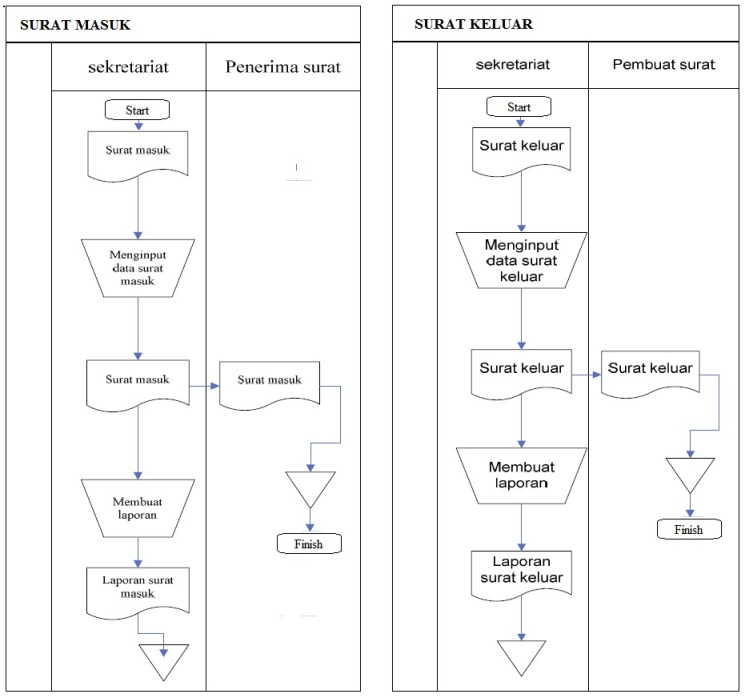
\includegraphics[width=12cm]{gambar/FlowchartAMSberjalan.png} 

Gambar 3.1 Flowchart Agenda Surat yang sedang berjalan


Sistem pencatatan agenda keluar masuk surat yang sedang berjalan pada umumnya telah memenuhi kebutuhan untuk pengolahan datanya, namun masih ada kekurangan pada beberapa proses seperti :
\begin{enumerate}
\item Kesulitan dalam proses pencarian data dan arsip surat masuk maupun data surat keluar.
\item Kesulitan dalam pembuatan laporan yang dikehendaki oleh perusahaan, karena data surat masuk dan surat keluar tidak tersimpan kedalam database.
\end{enumerate}

\section{Usulan Perancangan Sistem Aplikasi Manajemen Surat}
Tahapan selanjutnya adalah usulan perancangan sistem, hal ini dimaksudkan untuk mewujudkan perancangan sistem yang dibuat sesuai dengan kebutuhan.
Dari perancangan sistem yang diusulkan, peneliti prosedur yang diusulkan untuk membangun aplikasi agenda keluar masuk surat, yaitu:
\subsection{Flowchart}
Gambaran flowchart digambarkan sebagai berikut :

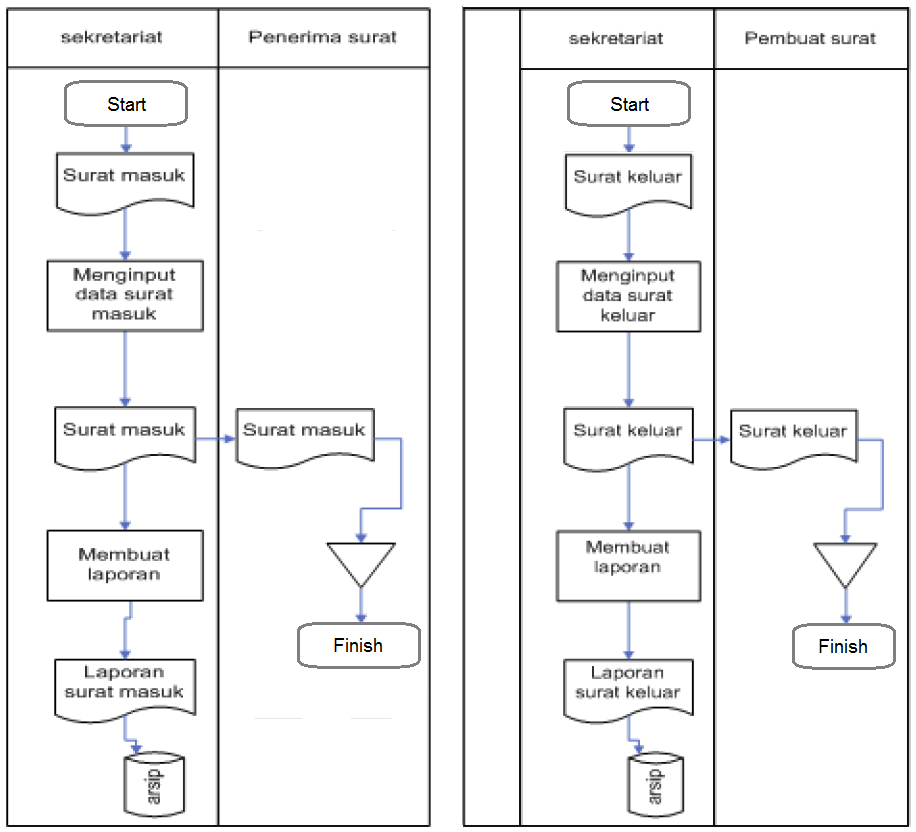
\includegraphics[width=11cm]{gambar/FlowchartAMSdiusulkan.png} 

Gambar 3.2 Flowchart aplikasi yang diusulkan

Alur kerja prosedur yang diusulkan untuk membangun aplikasi agenda keluar masuk surat yakni :

\begin{enumerate}
\item Bagian sekretariat menerima surat masuk dan surat keluar.
\item Kemudian sekretariat menginputkan data surat masuk dan surat keluar yang mengacu pada database agenda surat.
\item Setelah di input, bagian sekretariat menyerahkan form surat masuk dan surat keluar ke penerima surat.
\end{enumerate}

\subsection{Diagram Context}

berikut digambarkan diagram context dari aplikasi :

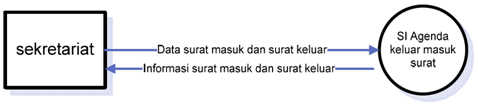
\includegraphics[width=13cm]{gambar/DiagramContext.png} 

Gambar 3.12 Diagram Context yang diusulkan

\subsection{DFD (Data Flow Diagram)}
berikut digambarkan DFD dari aplikasi :

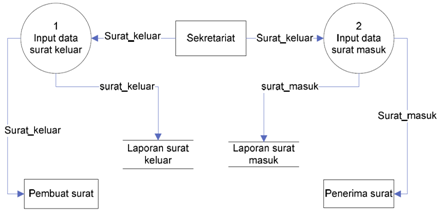
\includegraphics[width=13cm]{gambar/DFD.png}

Gambar 3.13 DFD (Data Flow Diagram) yang diusulkan

\section{Evaluasi Terhadap Sistem yang Diusulkan}
Sistem yang kami usulkan berupa sebuah aplikasi Agenda Surat Keluar Masuk. Aplikasi yang kami buat mempunyai kelebihan yaitu, diantaranya mempunyai penyimpanan data atau database yang baik. Aplikasi yang kami buat dapat memudahkan dalam penginputan data, pencarian data, pembuatan laporan. 

Aplikasi yang kami buat pun bersifat \textit{user friendly}, yang artinya aplikasi yang kami buat dapat mudah di jalankan oleh user tersebut. Aplikasi ini pun tidak memakan banyak waktu dan biaya karena telah dikemas kedalam sebuah aplikasi yang efisien.

\section{Jadwal Kegiatan}
Penelitian direncanakan akan dilaksanakan selama enam bulan. Rincian rencana jadwal penelitian dicantumkan dalam tabel berikut.

3.1 Tabel Jadwal Kegiatan Penelitian

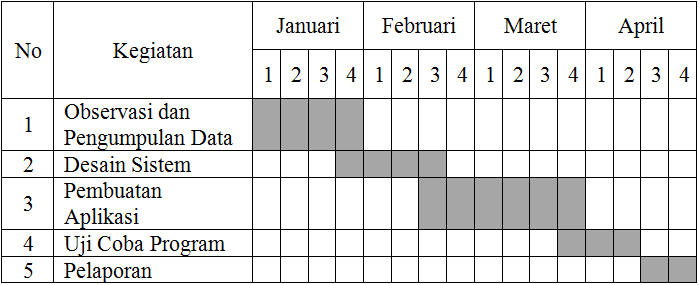
\includegraphics[width=13cm]{gambar/jadwal.png} 

%-----------------------------------------------------------------
%Disini akhir masukan Bab
%-----------------------------------------------------------------

%-----------------------------------------------------------------
%Disini awal masukan untuk Daftar Pustaka
%-----------------------------------------------------------------
%%\nocite{Abel2010,Guerbas201350}
%%\bibliography{research-plan}
%%\bibliographystyle{plainnat}
\begin{thebibliography}{9}

\bibitem[satu(2013)]{satu01}
Buku Profil Dinas Kesehatan Kabupaten Jember. 2014.

\bibitem[dua(2013)]{dua02}
Awan Pribadi Basuki, 2010,  Membangun Web Berbasis PHP Dengan Framework CodeIgniter, Lokomedia, Yogyakarta.

\bibitem[tiga(2013)]{tiga03}
Dodit Suprianto,  2008, Dasar Pemrograman PHP, OASE Media, Bandung.

\bibitem[empat(2013)]{empat04}
Eko Priyo Utomo, 2008, 125 Tips Menguasai Bahasa PHP, CV. Yramawidya, Bandung.

\bibitem[lima(2013)]{lima05}
Lukmanul Hakim, 2009,  Jalan Pintas Menjadi Master PHP, Lokomedia, Yogyakarta.

\bibitem[enam(2013)]{enam06}
Gamma,  Erich, 1995, Design Pattern: Element  of reusable object-oriented software, Addison-wisley.

\end{thebibliography}
\addcontentsline{toc}{chapter}{DAFTAR PUSTAKA}
%-----------------------------------------------------------------
%Disini akhir masukan Daftar Pustaka
%-----------------------------------------------------------------

\end{document}